\section{Evaluation}
\label{sec:evaluation}

\begin{figure*}[t!]
	\centering
	\begin{minipage}{.31\textwidth}
		\centering
		\subfloat[intra-host throughput]{                    
			%\begin{minipage}{0.4\textwidth}
			\centering
			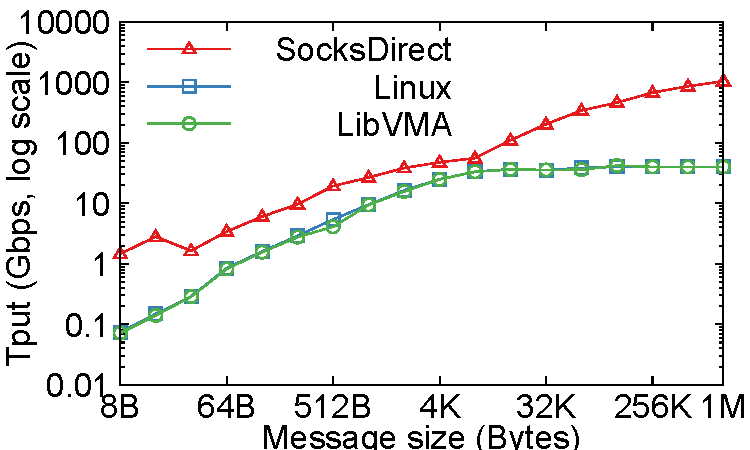
\includegraphics[width=\textwidth]{eval/microbenchmark/msgsize-ipc-tput.pdf}
			\label{fig:eval-msgsize-ipc-tput}
			%\end{minipage}
		}
		\vspace{-10pt}
		\subfloat[intra-host latency]{
			%\begin{minipage}{0.4\textwidth}
			\centering 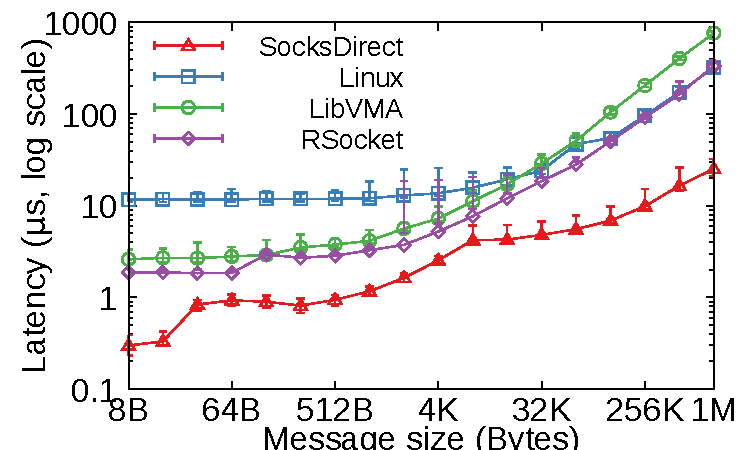
\includegraphics[width=\textwidth]{eval/microbenchmark/msgsize-ipc-lat.pdf}
			\label{fig:eval-msgsize-ipc-lat}
			%\end{minipage}
		}
		\vspace{-5pt}
		\caption{Single-core intra-host performance with message sizes.}
		\label{fig:eval-msgsize-intra}
	\end{minipage}
	\hspace{0.01\textwidth}
	\begin{minipage}{.31\textwidth}
		\centering
		\subfloat[inter-host throughput]{
			%\begin{minipage}{0.4\textwidth}
			\centering 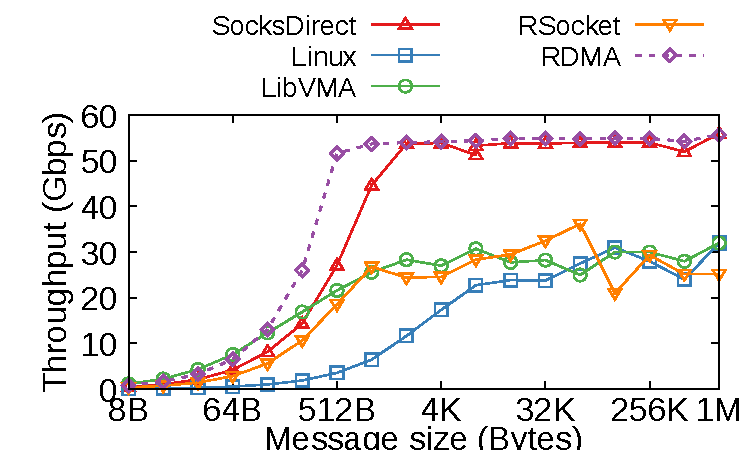
\includegraphics[width=\textwidth]{eval/microbenchmark/msgsize-network-tput.pdf}
			\label{fig:eval-msgsize-network-tput}
			%\end{minipage}
		}
		\vspace{-10pt}
		\subfloat[inter-host latency]{
			%\begin{minipage}{0.4\textwidth}
			\centering 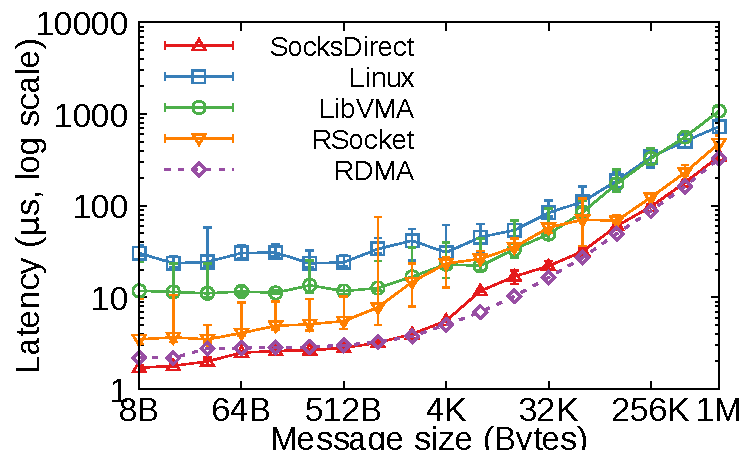
\includegraphics[width=\textwidth]{eval/microbenchmark/msgsize-network-lat.pdf}
			\label{fig:eval-msgsize-network-lat}
			%\end{minipage}
		}
		\vspace{-5pt}
		\caption{Single-core inter-host performance with message sizes.}
		\label{fig:eval-msgsize-inter}
	\end{minipage}
	\hspace{0.01\textwidth}
	\begin{minipage}{.31\textwidth}
		\subfloat[intra-host]{                    
			%\begin{minipage}{0.4\textwidth}
			\centering
			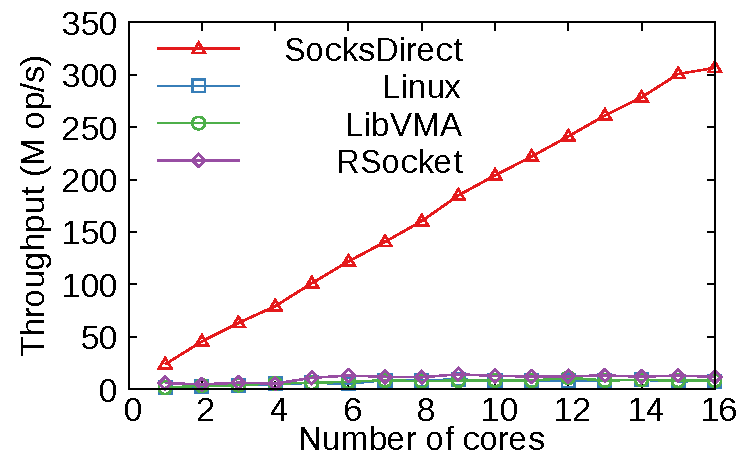
\includegraphics[width=\textwidth]{eval/microbenchmark/corenum-IPC-tput.pdf}
			\label{fig:eval-cornum-ipc}
			%\end{minipage}
		}
		\vspace{-5pt}
		\subfloat[inter-host]{
			%\begin{minipage}{0.4\textwidth}
			\centering 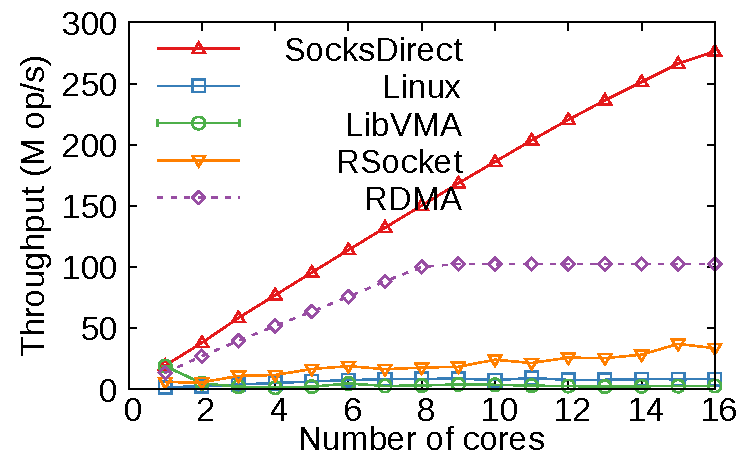
\includegraphics[width=\textwidth]{eval/microbenchmark/corenum-network-tput.pdf}
			\label{fig:eval-cornum-network}
			%\end{minipage}
		}
		\vspace{-5pt}
		\caption{Data transmission throughput with number of cores.}
		\label{fig:eval-corenum-tput}
	\end{minipage}
	\iffalse
	\begin{minipage}{.31\textwidth}
		\centering
		\subfloat[intra-host]{                    
			%\begin{minipage}{0.4\textwidth}
			\centering
			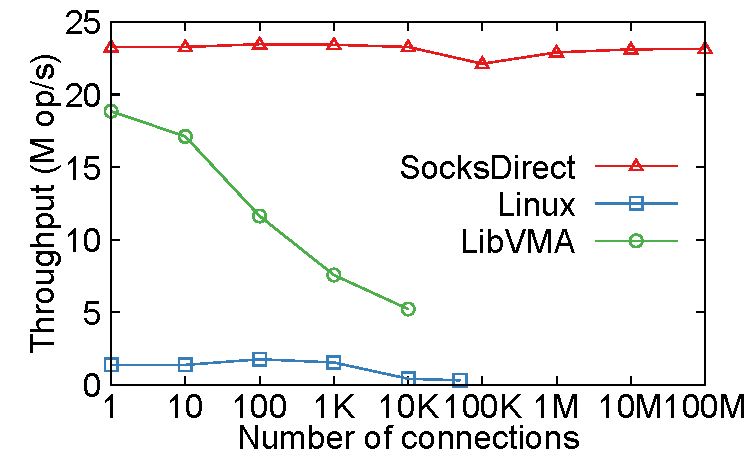
\includegraphics[width=\textwidth]{eval/microbenchmark/connnum-ipc-tput.pdf}
			\label{fig:eval-connnum-ipc-tput}
			%\end{minipage}
		}
		\vspace{-10pt}
		\subfloat[inter-host]{
			%\begin{minipage}{0.4\textwidth}
			\centering 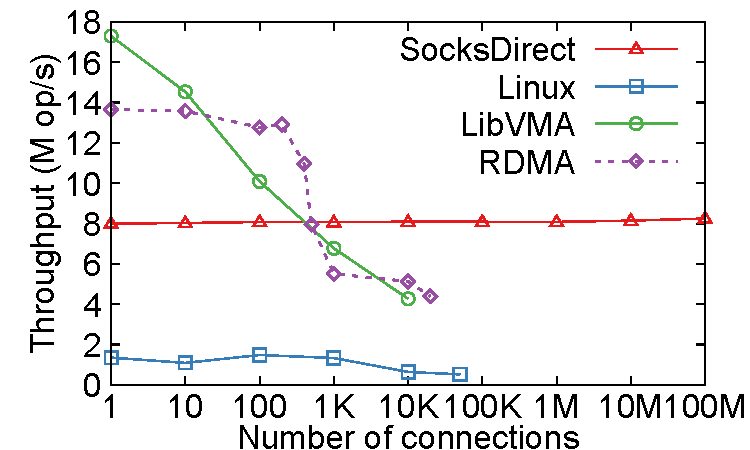
\includegraphics[width=\textwidth]{eval/microbenchmark/connnum-network-tput.pdf}
			\label{fig:eval-connnum-network-tput}
			%\end{minipage}
		}
		\vspace{-5pt}
		\caption{Single-core throughput with number of connections.}
		\label{fig:eval-connnum-tput}
	\end{minipage}
	\fi
\end{figure*}

%\begin{figure}[htpb]
%	\centering
%	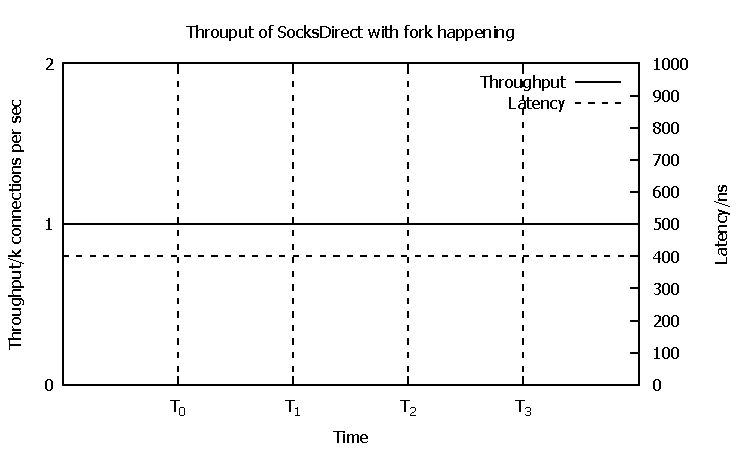
\includegraphics[width=\columnwidth]{eval/microbenchmark/fork-tput.pdf}
%	\caption{Throughput of SocksDirect with fork happening}
%	\label{fig:eval-fork-tput}
%\end{figure}

We implement \sys in three components: a user-space library \libipc{} and a monitor daemon with about 10K lines of C++ code, and a modified RDMA NIC driver to support zero copy.

We evaluate \sys in the following aspects:

\parab{Use shared memory efficiently for intra-host socket.}
For small messages, \sys achieves 0.3$\mu$s round-trip latency and up to 23~M messages per second throughput, close to raw shared memory performance. For large messages, \sys uses zero copy to achieve 13x lower latency and 26x throughput than Linux.

\parab{Use RDMA efficiently for inter-host socket.}
\sys achieves  1.7$\mu$s round-trip latency and 8M messages per second throughput, close to raw RDMA performance.

%\parab{Robust with number of connections.}
%The performance above can be maintained with up to 100 million connections.

\parab{Scale with number of cores.}
The performance above is linearly scalable with number of cores. %In addition, a single CPU core can create 1.4~M connections per second.

%\parab{Corner-case operations does not affect long-term performance.}
%After corner-case operations such as \texttt{fork}, the performance recovers quickly.




\subsection{Methodology}
\label{subsec:methodology}

We evaluate \sys on servers with two Xeon E5-2698 v3 CPUs, 256~GiB memory and a Mellanox ConnectX-4 NIC. Two servers are interconnected directly with 56~Gbps Ethernet cable. We use Ubuntu 16.04 with Linux 4.15, RoCEv2 for RDMA and poll completion queue every 64 messages.
Each thread is pinned on a CPU core. We run tests for enough warm-up rounds before collecting data. For latency, we report the mean, with error bars representing 1\% and 99\% percentile.
We compare with Linux and LibVMA~\cite{libvma}, a user-space TCP/IP stack optimized for Mellanox NICs.
This work does not raise any ethical issues.

\subsection{Microbenchmarks}
\label{subsec:microbenchmark}

\subsubsection{Latency and Throughput}
\quad



Figure~\ref{fig:eval-msgsize-intra} shows intra-host socket performance between a pair of sender and receiver threads.
For 8-byte messages, \sys achieves 0.3$\mu$s round-trip latency (35x lower than Linux) and 23~M messages per second throughput (20x Linux).
In comparison, a simple shared memory queue has 0.25$\mu$s round trip latency and 27~M throughput, indicating that \sys adds little overhead.
This latency is 5x lower than NIC hairpin, \textit{i.e.} one process sends packet to NIC and the NIC delivers it to another process. Using the NIC to forward intra-host packets involve PCIe latency.
The one-way delay of \sys is 0.15$\mu$s, even lower than a kernel crossing (0.2$\mu$s). Kernel-based sockets require a kernel crossing on both sender and receiver.

Due to memory copy, for 8~KiB messages, the throughput of \sys is only 60\% higher than Linux, and the latency is 4x lower. For messages larger than 8~KiB, \sys uses page remapping to achieve zero copy. For 1~MiB messages, \sys achieves 13x lower latency and 26x throughput than Linux.


Figure~\ref{fig:eval-msgsize-inter} shows inter-host socket performance between a pair of threads.
For 8-byte messages, \sys achieves 8M messages per second throughput (7x Linux) and 1.7$\mu$s round-trip latency (17x lower than Linux).
The throughput and latency is close to raw RDMA write operations (shown as dashed line), which does not have socket semantics.
LibVMA uses batching to achieve 19M throughput, but the latency is 7x of \sys.
For 2~KiB and larger messages, \sys saturates the network bandwidth, which is 2x of LibVMA and Linux. This performance gain mainly comes from zero copy.



\begin{figure*}[t!]
	\centering

	\hspace{0.01\textwidth}
	\begin{minipage}{.31\textwidth}
		%\centering
		%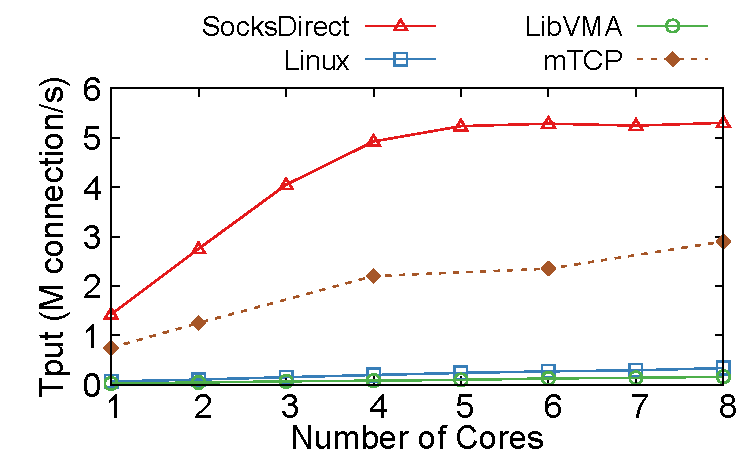
\includegraphics[width=\textwidth]{eval/microbenchmark/conn-setup-tput.pdf}
		%\vspace{-10pt}
		%\caption{Connection creation throughput with number of cores.}
		%\label{fig:eval-conn-setup-tput}
		
		%\begin{minipage}{0.4\textwidth}
		\centering 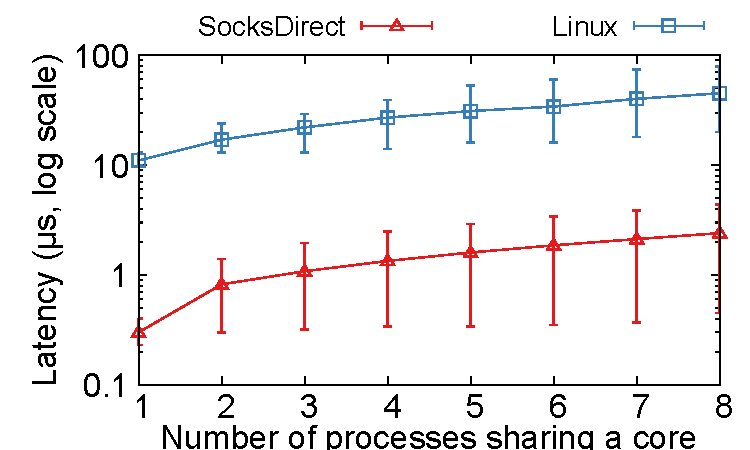
\includegraphics[width=\textwidth]{eval/microbenchmark/sharecore-lat.pdf}
		\vspace{-15pt}
		\label{fig:eval-context-switch}
		\caption{Latency of multiple processes sharing a core.}
		%\end{minipage}
	\end{minipage}
	\hspace{0.01\textwidth}
	\begin{minipage}{.31\textwidth}
		\centering
		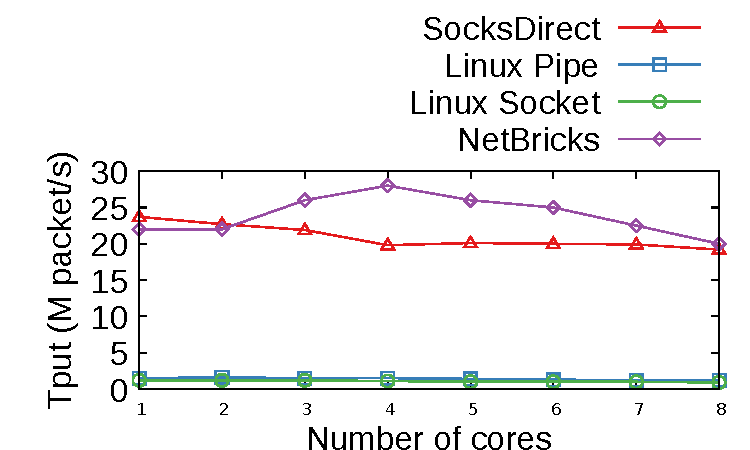
\includegraphics[width=\textwidth]{eval/microbenchmark/nfv-tun-tput.pdf}
		\caption{Throughput of NFV service chain.}
		\label{fig:eval-tun-tput}
		%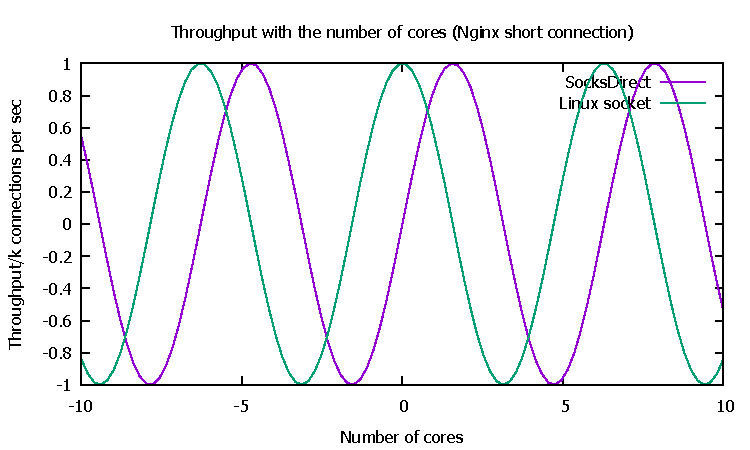
\includegraphics[width=\textwidth]{eval/microbenchmark/nginx-short-tput.pdf}
		%\vspace{-15pt}
		%\label{fig:eval-nginx-short}
		%\caption{Nginx throughput.}
		
		%\centering 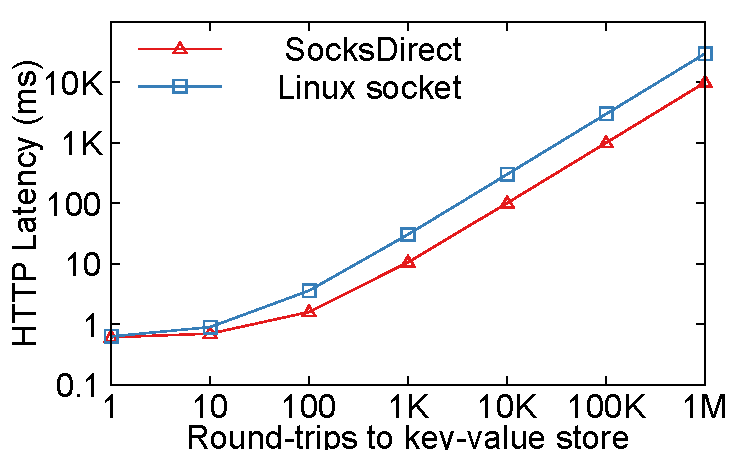
\includegraphics[width=\textwidth]{eval/microbenchmark/nginx-multiround-tput.pdf}
		%\vspace{-15pt}
		%\caption{End-to-end HTTP request latency of a web service.}
		%\label{fig:eval-nginx-multiround}
		
		%\centering
		%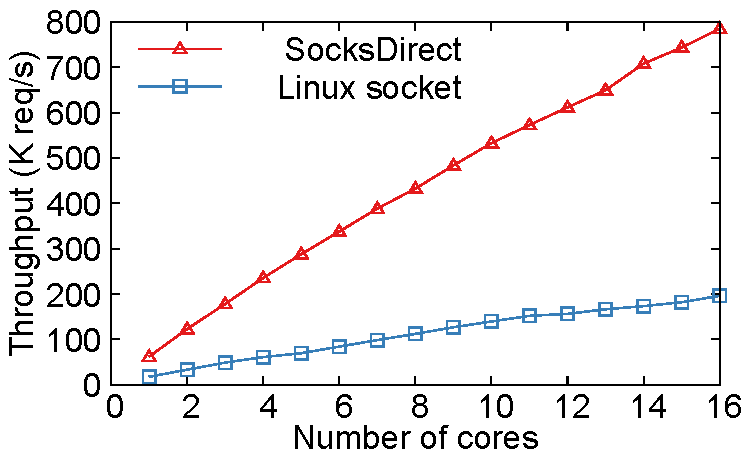
\includegraphics[width=\textwidth]{eval/microbenchmark/corenum-http-tput.pdf}
		%\vspace{-15pt}
		%\caption{Multi-core scalability of HTTP backend service throughput.}
		%\label{fig:eval-http-tput}
	\end{minipage}
\end{figure*}

\subsubsection{Multi-core Scalability}
\quad

%Figure~\ref{fig:eval-connnum-tput} shows the throughput with different number of concurrent connections.
%We establish connections between two processes before testing, then send and receive data from the connections in a round-robin order.
%\sys can support more than 100 million concurrent connections with 16~GiB of memory, and the throughput does not degrade under such high concurrency.
%\sys achieves connection stability by multiplexing connections via a single queue.
%In comparison, the performance of RDMA, LibVMA and Linux drops quickly as the number of connections increase. There is a sharp performance drop with more than 512 RDMA connections, because the RDMA transport states saturate the NIC cache. Although LibVMA and Linux do not use RDMA as transport, they maintain per-FD buffers, which lead to CPU cache and TLB miss with thousands of connections. Furthermore, LibVMA installs flow steering rules to NIC for each connection, which also leads to NIC cache miss.




Figure~\ref{fig:eval-corenum-tput} shows the throughput with different number of cores.
Sender and receiver process each creates several threads, then each thread pins on a core and communicates with a peer thread.
\sys achieves almost linear scalability for both intra-host and inter-host sockets.
For intra-host socket, \sys provides 306~M message per second throughput between 16 pairs of sender and receiver cores, which is 40x of Linux.
LibVMA falls back to Linux for intra-host socket.
Using RDMA for inter-host socket, \sys achieves 62~M messages per second throughput (8x Linux and 24x LibVMA).
Although \sys{} creates $n^2$ queues for $n$ sender and receiver threads, in this workload only $n$ of them are active.
Because the NIC only caches active RDMA connections and \libipc{} only polls active queues, the idle queues do not degrade performance.
Single thread LibVMA has better throughput than \sys due to batching.
Due to lock contention on shared NIC queues, compared to single thread, the throughput of LibVMA reduces to 1/4 with two threads, and 1/10 with three threads.
The Linux throughput scales linearly from 1 to 7 cores and bottlenecks on the loopback or NIC queues with more cores.
%The multi-thread scalability of \sys attributes to the partitioning of states and removal of synchronization.
%We can also see that shared memory communication has 5x throughput than RDMA.% Using RDMA NIC for intra-host socket would meet this bottleneck and thus not scalable.

%Figure~\ref{fig:eval-conn-setup-tput} shows the throughput of connection creation with different number of cores. Each core can create 1.4~M new connections per second, which is 20x of Linux and 2x of mTCP~\cite{jeong2014mtcp}. The upper bound is 5.3~M connections per second, where the monitor becomes a bottleneck.


Now we evaluate the performance of cooperative multitasking.
There may be multiple threads sharing a core, and each thread needs to wait for its turn to process messages.
Figure~\ref{fig:eval-context-switch} shows the message processing latency in such scenario.
First, when only a fraction of workers are active, the idle workers do not impact performance. 
Second, although the latency increases almost linearly with number of active workers, but it is still 20x to 30x lower than Linux, because cooperative context switch is faster than kernel wakeup.


%Finally, we benchmark the throughput and latency after \texttt{fork} and other corner-case operations. Initially, there is only one pair of sender and receiver. At time $T_0$, receiver forks, and the parent process keeps receiving. At time $T_1$, the child process begins to receives takes over the socket. At time $T_2$, sender forks, and only the parent sends. At time $T_3$, the child sender also starts sending. We find that both throughput and latency resume to initial maximal performance within 1~ms after each event.
